\documentclass[tikz,border=8mm]{standalone}
\usepackage[T1]{fontenc}
\usepackage{lmodern}
\usepackage{amsmath,amssymb}
\usetikzlibrary{arrows.meta,positioning,calc,decorations.pathreplacing}

\begin{document}
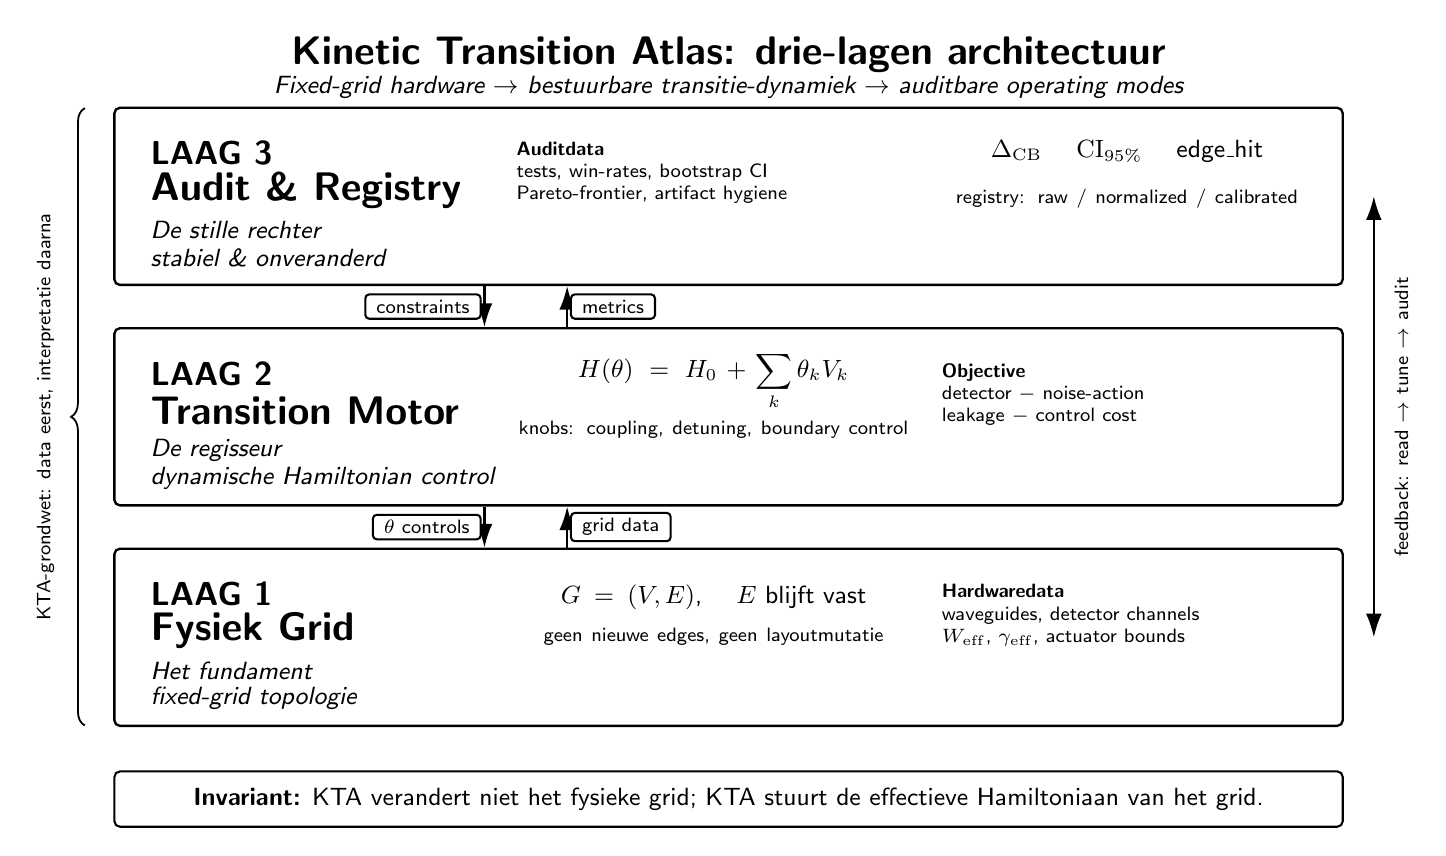
\begin{tikzpicture}[
  font=\sffamily,
  layerbox/.style={draw=black, rounded corners=2pt, line width=0.85pt,
                   minimum width=15.6cm, minimum height=2.25cm,
                   inner sep=0pt, fill=white},
  arrow/.style={-{Latex[length=3.0mm,width=2.0mm]}, line width=0.75pt},
  feedback/.style={{Latex[length=3.0mm,width=2.0mm]}-{Latex[length=3.0mm,width=2.0mm]}, line width=0.65pt},
  tag/.style={draw=black, rounded corners=1.4pt, inner xsep=4pt, inner ysep=2pt, font=\sffamily\scriptsize, fill=white},
  head/.style={font=\sffamily\bfseries\Large, align=left},
  sub/.style={font=\sffamily\itshape\small, align=left},
  micro/.style={font=\sffamily\scriptsize, align=left},
  mathnode/.style={font=\sffamily\small, align=center}
]

% Title
\node[font=\sffamily\bfseries\Large] at (0,5.15) {Kinetic Transition Atlas: drie-lagen architectuur};
\node[font=\sffamily\itshape\small] at (0,4.73) {Fixed-grid hardware $\rightarrow$ bestuurbare transitie-dynamiek $\rightarrow$ auditbare operating modes};

% Layer boxes
\node[layerbox] (L3) at (0,3.35) {};
\node[layerbox] (L2) at (0,0.55) {};
\node[layerbox] (L1) at (0,-2.25) {};

% Layer 3 content
\node[font=\sffamily\bfseries\large, anchor=west] at ($(L3.west)+(0.35,0.55)$) {LAAG 3};
\node[font=\sffamily\bfseries\Large, anchor=west] at ($(L3.west)+(0.35,0.08)$) {Audit \& Registry};
\node[font=\sffamily\itshape\small, anchor=west] at ($(L3.west)+(0.35,-0.42)$) {De stille rechter};
\node[font=\sffamily\itshape\small, anchor=west] at ($(L3.west)+(0.35,-0.78)$) {stabiel \& onveranderd};
\node[micro, text width=5.0cm, anchor=west] at ($(L3.west)+(5.00,0.30)$)
{\textbf{Auditdata}\\tests, win-rates, bootstrap CI\\Pareto-frontier, artifact hygiene};
\node[mathnode, text width=4.7cm, anchor=west] at ($(L3.west)+(10.40,0.28)$)
{$\Delta_{\mathrm{CB}}$ \quad $\mathrm{CI}_{95\%}$ \quad edge\_hit\\[2mm]
\scriptsize registry: raw / normalized / calibrated};

% Layer 2 content
\node[font=\sffamily\bfseries\large, anchor=west] at ($(L2.west)+(0.35,0.55)$) {LAAG 2};
\node[font=\sffamily\bfseries\Large, anchor=west] at ($(L2.west)+(0.35,0.08)$) {Transition Motor};
\node[font=\sffamily\itshape\small, anchor=west] at ($(L2.west)+(0.35,-0.42)$) {De regisseur};
\node[font=\sffamily\itshape\small, anchor=west] at ($(L2.west)+(0.35,-0.78)$) {dynamische Hamiltonian control};
\node[mathnode, text width=5.0cm, anchor=west] at ($(L2.west)+(5.00,0.28)$)
{$H(\theta)=H_0+\displaystyle\sum_k\theta_k V_k$\\[1mm]
\scriptsize knobs: coupling, detuning, boundary control};
\node[micro, text width=4.7cm, anchor=west] at ($(L2.west)+(10.40,0.28)$)
{\textbf{Objective}\\detector $-$ noise-action\\leakage $-$ control cost};

% Layer 1 content
\node[font=\sffamily\bfseries\large, anchor=west] at ($(L1.west)+(0.35,0.55)$) {LAAG 1};
\node[font=\sffamily\bfseries\Large, anchor=west] at ($(L1.west)+(0.35,0.08)$) {Fysiek Grid};
\node[font=\sffamily\itshape\small, anchor=west] at ($(L1.west)+(0.35,-0.42)$) {Het fundament};
\node[font=\sffamily\itshape\small, anchor=west] at ($(L1.west)+(0.35,-0.78)$) {fixed-grid topologie};
\node[mathnode, text width=5.0cm, anchor=west] at ($(L1.west)+(5.00,0.28)$)
{$G=(V,E)$, \quad $E$ blijft vast\\[1mm]
\scriptsize geen nieuwe edges, geen layoutmutatie};
\node[micro, text width=4.7cm, anchor=west] at ($(L1.west)+(10.40,0.28)$)
{\textbf{Hardwaredata}\\waveguides, detector channels\\$W_{\mathrm{eff}}$, $\gamma_{\mathrm{eff}}$, actuator bounds};

% Inter-layer arrows
\draw[arrow] ($(L3.south)+(-3.1,0)$) -- node[tag, midway, left=1pt] {constraints} ($(L2.north)+(-3.1,0)$);
\draw[arrow] ($(L2.north)+(-2.05,0)$) -- node[tag, midway, right=1pt] {metrics} ($(L3.south)+(-2.05,0)$);

\draw[arrow] ($(L2.south)+(-3.1,0)$) -- node[tag, midway, left=1pt] {$\theta$ controls} ($(L1.north)+(-3.1,0)$);
\draw[arrow] ($(L1.north)+(-2.05,0)$) -- node[tag, midway, right=1pt] {grid data} ($(L2.south)+(-2.05,0)$);

% Right-side feedback loop
\draw[feedback] ($(L1.east)+(0.38,0.0)$) -- ($(L2.east)+(0.38,0.0)$) -- ($(L3.east)+(0.38,0.0)$);
\node[rotate=90, font=\sffamily\scriptsize] at ($(L2.east)+(0.73,0.0)$) {feedback: read $\rightarrow$ tune $\rightarrow$ audit};

% Left-side brace
\draw[decorate, decoration={brace, amplitude=5pt}, line width=0.65pt]
  ($(L1.west)+(-0.36,-1.12)$) -- ($(L3.west)+(-0.36,1.12)$);
\node[rotate=90, font=\sffamily\scriptsize] at ($(L2.west)+(-0.86,0.0)$) {KTA-grondwet: data eerst, interpretatie daarna};

% Bottom invariant
\node[draw=black, rounded corners=2pt, line width=0.75pt, minimum width=15.6cm,
      inner sep=6pt, below=0.55cm of L1, align=center, font=\sffamily\small] (rule)
{\textbf{Invariant:} KTA verandert niet het fysieke grid; KTA stuurt de effectieve Hamiltoniaan van het grid.};

\end{tikzpicture}
\end{document}
